\documentclass[10pt]{extarticle}

\usepackage[utf8]{inputenc}              % Tipos de caracteres
\usepackage[portuguese]{babel}           % Português
\usepackage[a4paper,portrait]{geometry}  % Tipo de papel
\usepackage{color}                       % Para tratamento da cor
\usepackage{graphicx}                    % Para a imagem
\DeclareGraphicsExtensions{.jpg,.png}
\usepackage{amsmath}                     % Para as matematiquices
\usepackage{amssymb}
\usepackage{array}
\usepackage{gensymb}                     % Grau
\usepackage{multicol}
\setlength{\columnsep}{1cm}
\usepackage{geometry}					% Margens
%\usepackage{xfrac}
\usepackage{colortbl}

\usepackage{multirow}

\addtolength{\topmargin}{-28mm}
\addtolength{\textheight}{62mm}
\addtolength{\oddsidemargin}{-15mm}
\addtolength{\textwidth}{32mm}

\renewenvironment{abstract}
 {\small
  \begin{center}
  \bfseries \abstractname\vspace{-.5em}\vspace{0pt}
  \end{center}
  \list{}{
    \setlength{\leftmargin}{0cm}%
    \setlength{\rightmargin}{\leftmargin}%
  }%
  \item\relax}
 {\endlist}
 
\renewcommand{\abstractname}{Resumo}

\delimitershortfall-1sp
\newcommand\abs[1]{\left|#1\right|}
\newcommand{\PR}[1]{\ensuremath{\left[#1\right]}}
\newcommand{\PC}[1]{\ensuremath{\left(#1\right)}}
\newcommand{\chav}[1]{\ensuremath{\left\{#1\right\}}}

\newcolumntype{x}[1]{>{\centering\hspace{0pt}}p{#1}}

\begin{document}

\title {\bf \huge T0 - Caracterização de uma Célula Fotovoltaica}
\author
{{\small Grupo III - João Ferreira (78179) Henrique Rodrigues (78632) Rodrigo C. Carvalho (78646) Cristina Melício (78947)} \\
{\small MEFT - 2ºAno, 2º Semestre - Laboratório de Complementos de Eletromagnetismo e Termodinâmica}}
\date{{\small Sexta-Feira, 27 de Fevereiro de 2015 \\ Sexta-Feira, 6 de de Março de 2015}}
\maketitle

\begin{abstract}
\par O objectivo deste trabalho experimental foi a determinação da característica eléctrica e da resistência de carga óctima que maximiza a potência eléctrica da célula fotovoltaica, para diferentes níveis de iluminação.
Verificou-se ainda que as grandezas que variam linearmente com o nível de iluminação são a intensidade de corrente e a potência máxima.
Por fim, descobriu-se um modelo que relaciona a variação da potência com $d^{-2.78}$, sendo $d$ a distância à fonte luminosa.
\end{abstract}

\begin{multicols}{2}

\section{Introdução}

\par A actividade laboratorial consiste no estudo da característica eléctrica duma célula fotovoltaica, através do circuito eléctrico apresentado na figura 1:

\hspace{-0.8cm}
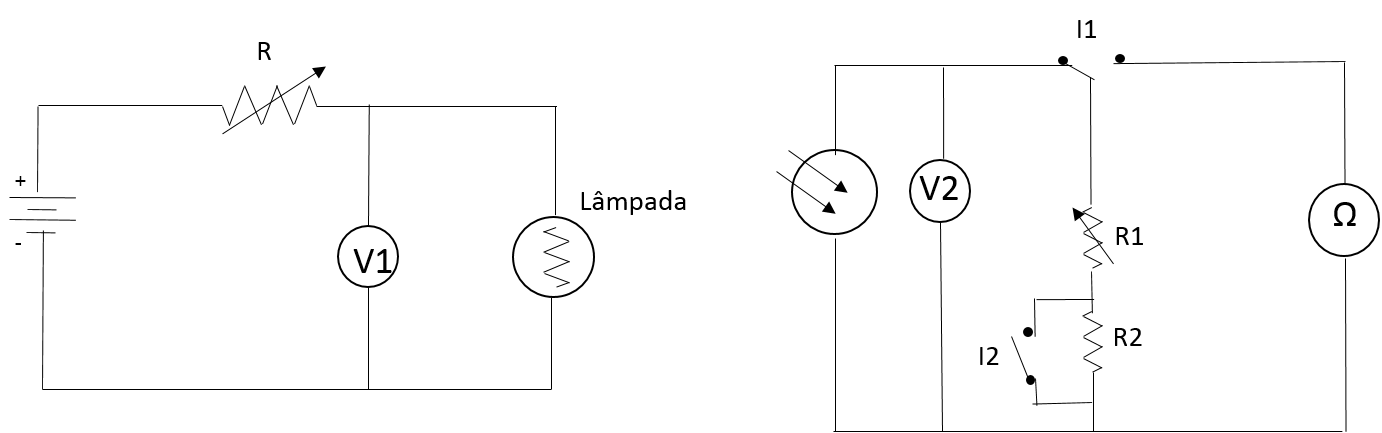
\includegraphics[width=260pt]{circuito}
\begin{center}
\par\noindent {\scriptsize (Figura 1: Esquema da montagem)}
\end{center}

\par Uma célula fotovoltaica, por definição, permite a conversão directa de energia luminosa em energia eléctrica e o seu funcionamento é semelhante ao efeito fotoeléctrico. Assim, é composta por duas camadas de materiais semicondutores dopadas de forma diferente. Entre a camada N, onde existe um excesso de eletrões periféricos e a camada P, onde existe um défice dos mesmos, cria-se uma diferença de potencial que produz uma corrente contínua no circuito ligado à célula. Esta irá ser responsável pelo surgimento de uma corrente no circuito, possibilitando por conseguinte o estudo das relações entre a iluminação proporcionada pela lâmpada e os valores das diversas grandezas cujo estudo constitui o âmbito deste trabalho. 

\par Caso o circuito alimentado pela célula fotovoltaica seja um circuito resistivo, isto é, um circuito simples composto apenas por resistências eléctricas, a intensidade pode ser obtida através da Lei de Ohm, uma vez conhecidas a resistência total do circuito e a tensão nos terminais da célula:

\begin{equation} \label{eq1}
U=RI \Leftrightarrow I=\frac{U}{R}
\end{equation}

\par A potência eléctrica, por sua vez, é obtida pela Lei de Joule através de outra relação entre a resistência e a tensão:
\begin{equation} \label{eq2}
P=UI=\frac{U^2}{R}
\end{equation}

\par
A intensidade luminosa incidente na célula fotovoltaica depende de diversos factores tais como a inclinação da superfície da célula em relação à fonte de luz. Por isso, considera-se a seguinte relação de proporcionalidade, em que I é o nível de iluminação em percentagem:

\begin{equation}
I\propto\cos{\alpha}
\end{equation}

\par Outros factores em relação aos quais também se verifica uma dependência da intensidade luminosa incidente na célula fotovoltaica são, por exemplo, a distância da célula à fonte e naturalmente a própria potência da fonte. É de salientar que, para uma propagação de geometria esférica ou cónica, a intensidade decai com o quadrado da distância à fonte luminosa, isto é, I \propto \frac{1}{d^2}

%\section{Diagrama de Blocos}
%\par Cenas

\section{Dados Experimentais}

\subsection*{\normalsize Característica eléctrica da célula fotovoltaica}

\par Depois de efetuar a montagem do circuito de acordo com o indicado no protocolo, procedeu-se à determinação da característica elétrica da célula fotovoltaica, isto é, da relação tensão-corrente.

\par Para tal, fazendo uso dos interruptores 1 e 2 e da caixa de resistências, fez-se variar a resistência $R$ indicada no Ohmímetro em intervalos de aproximadamente $100\Omega$. Para cada valor, leu-se no voltímetro e registou-se o valor da diferença de tensão $U$ entre os terminais da célula fotovoltaica e calculou-se o valor da intensidade de corrente $I$ através da Lei de Ohm, descrita na equação \eqref{eq1}.

\par Este procedimento foi repetido para os ângulos $\alpha$ de inclinação da célula $0^\circ$, $20^\circ$, $40^\circ$, $60^\circ$ tendo-se obtido os seguintes resultados:

\begin{center}
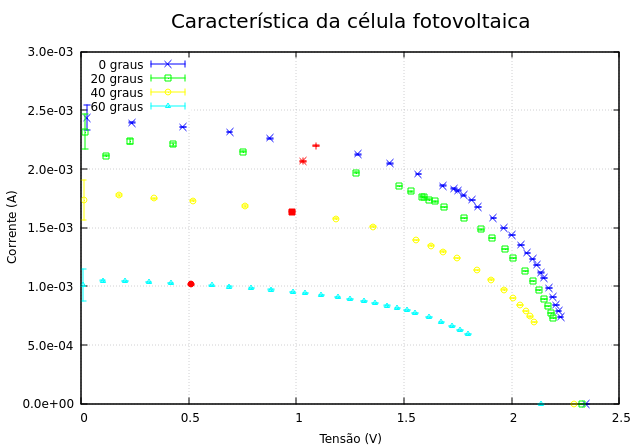
\includegraphics[width=240pt]{I-Vgrid2}
\par\noindent {\scriptsize ({\bf Gráfico 1}: Pontos experimentais referentes aos valores da corrente como função da tensão entre os terminais da célula fotovoltaica. De cima para baixo, encontram-se a vermelho os pontos $(1.090V,2.198mA)$, $(1.031V,2.066mA)$, $(0.980V,1.636mA)$, $(0.510V,1.018mA)$)
\end{center}

\subsection*{Resistência de carga ótima}

\par Calculou-se a potência através da expressão \eqref{eq2}. No seguinte gráfico representam-se os valores da potência em função da resistência, referentes a cada um dos ângulos estudados anteriormente:

\begin{center}
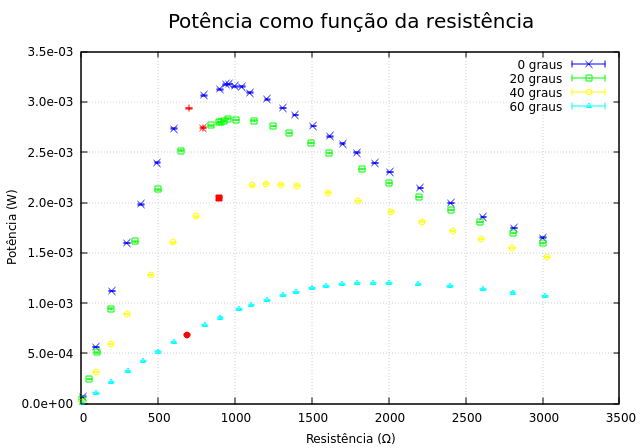
\includegraphics[width=240pt]{P-Rgrid2}
\par\noindent {\scriptsize ({\bf Gráfico 2}: Pontos experimentais referentes aos valores da potência em função da resistência. De cima para baixo, encontram-se a vermelho os pontos $(700\Omega,2.938mW)$, $(796\Omega,2.744mW)$, $(899\Omega,2.048mW)$, $(690\Omega,0.688mW)$)}
\end{center}

\par\noindent Para cada caso, efetuando a média entre os dois pontos com potência mais elevada, encontrou-se o máximo de potência $P_{max}$, cujo maximizante $R_{max}$ corresponde à resistência de carga ótima. Na seguinte tabela apresentam-se os resultados:

{\small
\begin{center}
\begin{tabular}{ x{1.7cm} x{2cm} x{2.5cm} }
$\alpha$ ($^\circ$) & $P_{max}$ ($mW$) & $R_{max}$ ($\Omega$) \tabularnewline
\hline \hline
0  & 3.176$\pm$0.002 & (9.5$\pm$0.1)$\times10^2$ \tabularnewline
20 & 2.828$\pm$0.006  & (9.8$\pm$0.3)$\times10^2$ \tabularnewline
40 & 2.184$\pm$0.005 & (1.25$\pm$0.05)$\times10^3$ \tabularnewline
60 & 1.203$\pm$0.001 & (1.95$\pm$0.05)$\times10^3$ \tabularnewline
\end{tabular}
\par\noindent {\scriptsize ({\bf Tabela 1}: Valores da potêcia máxima para cada ângulo e respetiva resistência de carga ótima)}
\end{center}
}

\subsection*{Relações de linearidade}

\par Pretendia-se analisar a variação de certas grandezas com o nível de iluminação da célula fotoelétrica, sendo este dado pelo cosseno do ângulo de inclinação.

\begin{itemize}

\item \textbf{Corrente com tensão fixa $U_0=1.7V$}
\par Para cada ângulo, efetuou-se uma interpolação linear entre os valores da corrente dos dois pontos com tensão imediatamente interior e superior a $U_0$. Os resultados obtidos encontram-se na tabela 2 e no gráfico 3:

{\small
\begin{center}
\begin{tabular}{ x{1.5cm} x{1.5cm} x{1.9cm} }
$\alpha$ ($^\circ$) & $\cos{\alpha}$ (\%) & $I$ ($mA$) \tabularnewline
\hline \hline
0  & 100.0 & 1.850$\pm$0.004 \tabularnewline
20 & 94.0  & 1.660$\pm$0.004 \tabularnewline
40 & 76.6  & 1.280$\pm$0.003 \tabularnewline
60 & 50.0  & 0.677$\pm$0.002 \tabularnewline
\end{tabular}
\par\noindent {\scriptsize ({\bf Tabela 2}: Valores da corrente para cada ângulo para uma tensão de $1.7V$)}
\end{center}
}

\vspace{-0.8cm}

\begin{center}
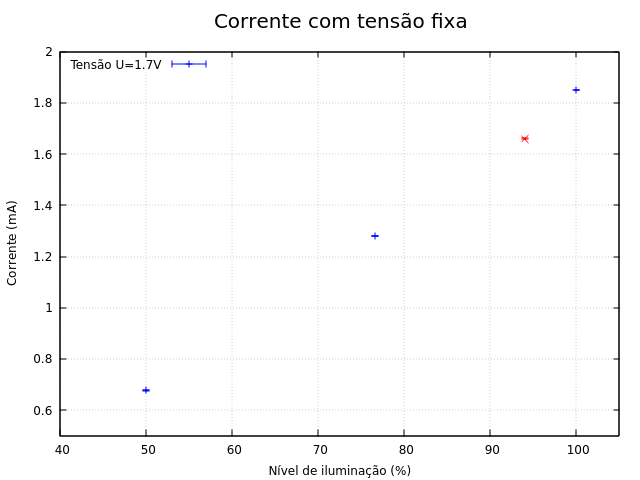
\includegraphics[width=240pt]{Tfixa}
\par\noindent {\scriptsize ({\bf Gráfico 3}: Valores da corrente representados em função do nível de iluminação, para uma tensão de $1.7V$. A vermelho indica-se o ponto $(94.0\%,1.660mA)$)}
\end{center}

\item \textbf{Tensão com corrente nula}

\par Utilizaram-se os pontos que se encontram sobre o eixo 0x no gŕafico 1, que foram obtidos abrindo o circuito no interruptor I1.

{\small
\begin{center}
\begin{tabular}{ x{1.5cm} x{1.5cm} x{2cm} }
$\alpha$ ($^\circ$) & $\cos{\alpha}$ (\%) & $U$ ($V$) \tabularnewline
\hline \hline
0  & 100.0 & 2.345$\pm$0.001 \tabularnewline
20 & 94.0  & 2.327$\pm$0.001 \tabularnewline
40 & 76.6  & 2.290$\pm$0.001 \tabularnewline
60 & 50.0  & 2.136$\pm$0.001 \tabularnewline
\end{tabular}
\par\noindent {\scriptsize ({\bf Tabela 3}: Valores da tensão para cada ângulo para uma corrente nula)}
\end{center}
}

\begin{center}
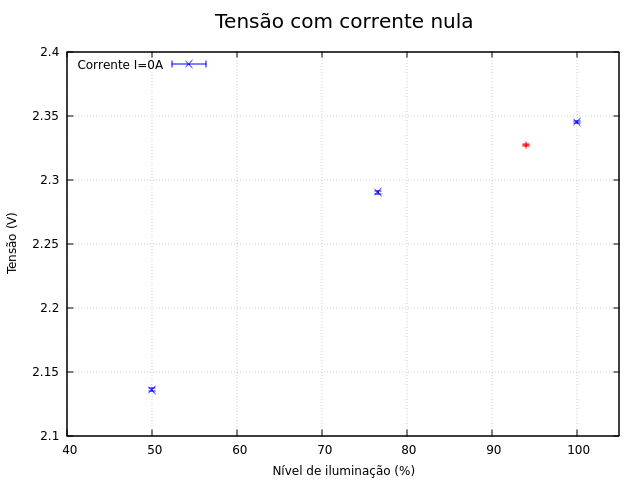
\includegraphics[width=240pt]{Izero}
\par\noindent {\scriptsize ({\bf Gráfico 4}: Valores da tensão representados em função do nível de iluminação, para uma corrente nula. A vermelho indica-se o ponto $(94.0\%,2.327V)$)}
\end{center}

\item \textbf{Potência com resistência fixa $R_0=1250\Omega$}
\par Para cada ângulo, efetuou-se uma interpolação linear entre os valores da potência dos dois pontos com resistência imediatamente interior e superior a $R_0$. Os resultados obtidos encontram-se na tabela 4 e no gráfico 5:

{\small
\begin{center}
\begin{tabular}{ x{1.5cm} x{1.5cm} x{2cm} }
$\alpha$ ($^\circ$) & $\cos{\alpha}$ (\%) & $P$ ($mW$) \tabularnewline
\hline \hline
0  & 100.0 & 2.994$\pm$0.007 \tabularnewline
20 & 94.0  & 2.759$\pm$0.006 \tabularnewline
40 & 76.6  & 2.184$\pm$0.005 \tabularnewline
60 & 50.0  & 1.053$\pm$0.004 \tabularnewline
\end{tabular}
\par\noindent {\scriptsize ({\bf Tabela 4}: Valores da potência para cada ângulo para uma resistência de $1250\Omega$)}
\end{center}
}

\begin{center}
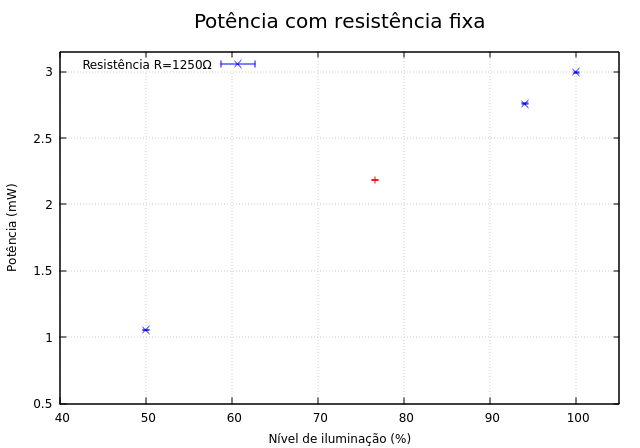
\includegraphics[width=240pt]{Rfixa}
\par\noindent {\scriptsize ({\bf Gráfico 5}: Valores da potência representados em função do nível de iluminação, para uma resistência de $1250\Omega$. A vermelho indica-se o ponto $(76.6\%,2.184mW)$)}
\end{center}

\item \textbf{Valor da resistência de carga ótima}

\par Representaram-se os valores da terceira coluna da tabela 1 no gráfico 6:

\begin{center}
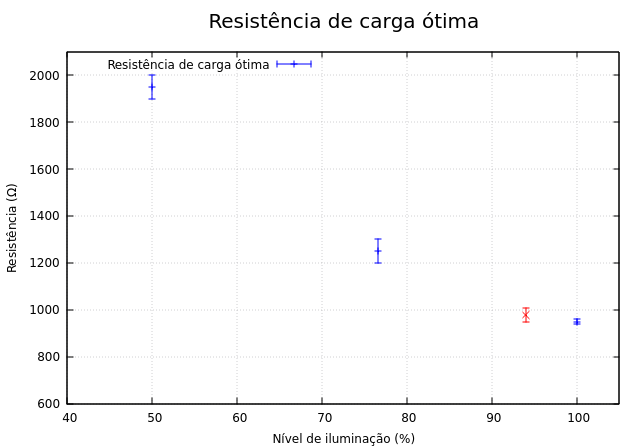
\includegraphics[width=240pt]{Rotima}
\par\noindent {\scriptsize ({\bf Gráfico 6}: Valores da resistência de carga ótima representados em função do nível de iluminação. A vermelho indica-se o ponto $(94.0\%,980\Omega)$)}
\end{center}

\item \textbf{Valor da potência máxima}

\par Representaram-se os valores da segunda coluna da tabela 1 no gráfico 7:

\begin{center}
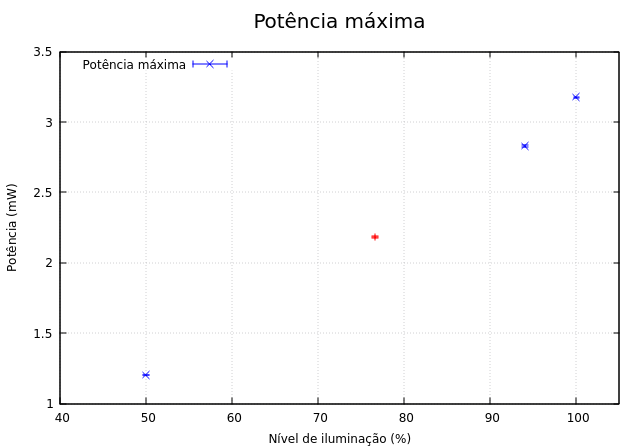
\includegraphics[width=240pt]{Pmax}
\par\noindent {\scriptsize ({\bf Gráfico 7}: Valores da potêcia máxima representados em função do nível de iluminação. A vermelho indica-se o ponto $(76.6\%,2.184mW)$)}
\end{center}

\end{itemize}

\subsection*{Variação da potência com a distância}

\par Nesta secção, pretendia-se analisar a variação da potência fornecida à carga pela célula fotovoltaica com a distância desta à fonte luminosa.

\par Para tal, variámos a referida distância, mantendo constante uma resistência de $R=(2.003\pm0.001)k\Omega$, e medindo o valor da tensão nos terminais da célula correspondente. Assim, através da expressão \eqref{eq2} foi possível obter valores de potência como função da potência. É necessário notar apenas que, estando a célula e a fonte encostadas, o valor de distância indicado na régua é ainda $d_0=(0.052\pm0.001)m$, tendo portanto sido necessário descontar este valor aos medidos. No seguinte gráfico 8 apresenta-se o logaritmo da potência como função do logaritmo da distância:

\begin{center}
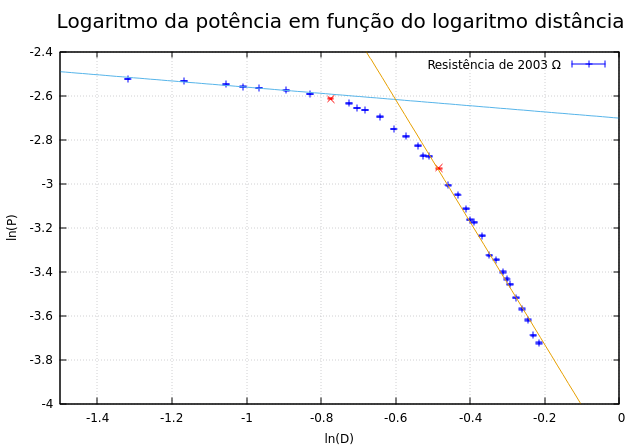
\includegraphics[width=240pt]{lnP-lnD}
\par\noindent {\scriptsize ({\bf Gráfico 8}: Representação de $\log{P}$ como função de $\log{d}$. Da esquerda para a direita indicam-se a vermelho os pontos $(-0.775,-2.613)$ e $(-0.484,-2.929)$)}
\end{center}

\par A estes pontos ajustou-se pelo método dos mínimos quadrados dois regimes lineares da forma

\begin{equation}
\log{P} = a\log{d}+b
\end{equation}

\par\noindent aos intervalos $I_A=[-1.4;-0.80]$ e $I_B=[-0.55;-0.2]$, tendo-se obtido os seguintes resultados:

\begin{center}
\begin{tabular}{ x{0.7cm} x{0.7cm} x{2cm}}
\hline \hline
\multirow{2}{*}{$I_A$} & $a$ & -0.14$\pm$0.02 \tabularnewline
 & $b$ & -2.70$\pm$0.02 \tabularnewline
\multirow{2}{*}{$I_B$} & $a$ & -2.78$\pm$0.07 \tabularnewline
 & $b$ & -4.29$\pm$0.03 \tabularnewline
\hline \hline
\end{tabular}
\end{center}

\par De seguida, analisou-se a variação da potência máxima com a distância entre a célula fotovoltaica e a fonte luminosa, tendo-se obtido os seguintes resultados:

{\small
\begin{center}
\begin{tabular}{ x{1.7cm} x{2.2cm} x{2.5cm} }
$d$ ($m$) & $P_{max}$ ($mW$) & $R_{max}$ ($\Omega$) \tabularnewline
\hline \hline
0.148 & 5.2586$\pm$0.0006 & (9.5$\pm$0.1)$\times10^2$ \tabularnewline
0.198 & 3.31$\pm$0.06  & (9.8$\pm$0.3)$\times10^2$ \tabularnewline
0.248 & 2.064$\pm$0.002 & (1.25$\pm$0.05)$\times10^3$ \tabularnewline
\end{tabular}
\par\noindent {\scriptsize ({\bf Tabela 5}: Valores da potêcia máxima para diferentes distâncias e respetiva resistência de carga ótima)}
\end{center}
}

\section{Discussão dos Resultados}

\par Relativamente à curva característica do circuito foi possível constatar que a um aumento do ângulo correspondia uma diminuição da intensidade luminosa fornecida e uma subsequente diminuição da intensidade de corrente, o que é lógico: uma menor intensidade luminosa leva a um menor excitamento dos electrões presentes na célula fotovoltaica e, como tal, a uma menor intensidade de corrente. De facto, tal é corroborado pelo máximo da intensidade da corrente ser tão maior quão menor é a inclinação considerada. A análise efectuada para uma quantidade suficientemente vasta de valores de resistências permite, além disso, comparar o comportamente da curva característica para os diversos ângulos de forma mais pormenorizada, possibilitando constatar que, para ângulos menos elevados, a valores elevados de resistências o decréscimo do valor da intensidade em função do aumento da resistência (o declive da curva) é demarcadamente mais pronunciado.

\par No tocante à segunda parte da experiência é facilmente observável, mediante a análise do gráfico elaborado, que o valor da potência máxima é tão maior quão maior for a intensidade luminosa, isto é, quão menor for o ângulo considerado, e que o valor da resistência de carga óptima é tão menor quão maior for a intensidade luminosa, isto é, quão menor for o valor do ângulo considerado. É de salientar que tanto o valor da resistência de carga óptima como o da potência máxima possuem um elevado grau de precisão porquanto foi progressivamente aproximado, sendo considerado um número mais significativo de dados em torno do valor máximo da potência do que nos restantes por forma a garantir uma maior precisão na sua determinação. Além disto, devemos ainda mencionar que quão maior for o ângulo de inclinação considerado, isto é, quão menor a intensidade luminosa, maior é a zona na qual a potência máxima varia pouco, ou seja, existe um maior conjunto de valores de resistências tais que o valor da potência varie de forma menos significativa, tornando mais difícil a identificação da resistência de carga óptima.

\par Quanto à linearidade das grandezas em estudo, pode verificar-se imediatamente pela análise directa dos gráficos que a intensidade de corrente varia linearmente com a intensidade luminosa, ao contrário da tensão. Por outro lado, a potência para um valor de resistência fixa evidencia a forma quadrática esperada de forma evidente, mas não se revela tão claramente linear quanto as restantes, pelo que seria necessário obter mais amostragens experimentais para obter uma conclusão absoluta, embora o formato do gráfico indicie uma relação não-linear. A resistência de carga óptima, por seu lado, é claramente não-linear. Todavia, o valor da potência máxima parece apresentar uma relação de linearidade em relação à intensidade luminosa. Notemos que para garantir uma maior qualidade na extrapolação destas relações seria forçoso efectuar medições para percentagens de intensidade luminosa inferiores àquelas consideradas, isto é, ângulos maiores, possibilitando um maior conjunto de dados a partir dos quais extrair as inferências necessárias.

\par Por fim, no que é pertinente à relação entre a distância e a intensidade luminosa revela-se forçoso analisar o gráfico obtido em função de dois regimes distintos. O primeiro regime diz respeito a distâncias particularmente pequenas entre a célula fotovoltaica e a lâmpada, para o qual se obteve um declive de valor $a=-0.14\pm0.02$. Para este regime, a grande aproximação à fonte luminosa permite efectuar uma aproximação a uma fonte pontual de luz, isto é, esperar-se-ia que o valor da intensidade luminosa, no âmbito dessa aproximação, não variasse com a distância - de facto, uma lei potencial não seria adequada em virtude da própria forma do gráfico. E, de facto, para as distâncias consideradas, o baixo valor do declive da recta indicia que esta aproximação possui mérito. Todavia, esta aproximação torna-se absolutamente errónea a partir de distâncias mais elevadas (cerca de 10 cm), vendo-nos forçados a considerar uma fonte luminosa tal que a luz emitida possuirá uma uma propagação de geometria esférica, ou seja, a intensidade da luz emitida decairá com o quadrado da distância à fonte luminosa. Notamos ademais que esta distância e a variação de regime que lhe está intrínseca resulta da não-trivialidade da forma da lâmpada, a qual leva à existência de um foco a esta distância que será o principal responsável pela mudança de reigmes evidenciada.

\par De facto, para o segundo regime, obteve-se um declive de $a=-2.78\pm0.07$. Todavia, visto a intensidade de corrente variar linearmente com a intensidade luminosa e a potência variar com o quadrado da intensidade de corrente, poder-se-ia esperar que a potência decaísse com a quarta potência da distância. Isto seria verdade para valores de resistência muito diferentes dos da resistência óptima. Como contudo utilizámos um valor de resistência elevado, da ordem dos $2k\ohm$, sabemos a partir da tabela 5 que a resistência óptima irá ser atingida para distâncias mais elevadas, que correspondem ao regime estudado. Além disso, o elevado valor da resistência de carga óptima para estas distâncias relaciona-se com o facto de a potência máxima ser menos acentuada, isto é, para variações em torno da resistência óptima verificam-se menores variações dos valores de potência correspondentes (tal como é evidenciado por uma parte anterior deste mesmo trabalho). Portanto, para o conjunto das distâncias avaliadas, o valor das potências não se afastará em demasia do valor da potência máxima, garantindo consequentemente uma variação quadrática com a distância. A variação nunca será exactamente quadrática porque a resistência fixa significa que à medida que estudamos distâncias cujo valor é mais distinto daquela para o qual a resistência utilizada corresponde à resistência de carga óptima a variação da potência em relação à potência máxima para essa distância será mais acentuada, levando a que varie expectavelmente com um valor um pouco superior ao quadrado da distância. E, de facto, é isso que se verifica, como evidenciado pelo declive da recta cujo valor foi acima explicitado.

\par Assim, para o primeiro regime não se considera uma lei de potência enquanto que no tocante ao segundo regime se considera uma lei cuja forma será dada pela expressão $P=\frac{C}{d^{2.78}}$, onde $C\in\mathbb{R}$.

\section{Conclusão}

\par Após a realização da experiência, foi possível extrair diversas ilações. 

\par Em primeiro lugar, concluiu-se que em relação às fontes de erro, estas provenieram maioritariamente de problemas de orientação da lâmpada em relação à célula fotovoltaica e de problemas de ruido luminoso, no sentido em que, apesar de as luzes do tecto da sala onde se realizou a experiência se encontrarem apagadas, ainda existirem uma míriade de outras fontes luminosas cuja interferência sistemática com a experiência constitui um erro impossível de eliminar e onde radica grande parte dos desvios da experiência em relação aos valores esperados. Além do mais, considera-se que seria vantajoso considerar distâncias maiores que aquelas permitidas pela calha, a qual apenas permitia medir valores até 75 cm, porquanto isto possibilitaria a utilização de ângulos maiores e, consequentemente, o estudo de resistência da carga óptima para menores valores de intensidade luminosa.

\par Relativamente às curvas características, verificou-se que a uma maior inclinação da célula corresponde uma menor intensidade máxima de corrente e um valor menor de tensão para o qual a intensidade tende para zero. Quanto a relações de linearidade, verifica-se que tanto a intensidade de corrente quanto a potência máxima eram as únicas grandezas que variavam linearmente com a intensidade luminosa. Por fim, verifica-se que existem dois regimes relativamente à potência. O primeiro, para distâncias pequenas, não apresenta uma lei de potências; o segundo, por outro lado, apresenta uma lei de $d^{-2.78}$.


\end{multicols}

\begin{thebibliography}{9}

\bibitem{guia} Guia de objetivos do trabalho, Professor João Figueirinhas
\bibitem{apontamentos} Apontamentos das aulas teóricas
\bibitem{site}  \url{http://en.wikipedia.org/wiki/thermoelectric\_effect}
\end{thebibliography}

\end{document}

% FOTOGRAFIA
%\begin{center}
%\includegraphics[width=240pt]{NOME SEM EXTENSAO}
%\par\noindent {\scriptsize (Figura X: Descrição)}
%\end{center}

%NOVA SUBSECÇÃO
%\subsection*{\normalsize BLA BLA}

%TABELA
%\begin{center}
%\begin{tabular}{ x{1.5cm} ... }
%i & ... \tabularnewline
%\hline \hline
%1 & 4.15  & 0.15  & 2033 & -  \tabularnewline
%\end{tabular}
%\par\noindent {\scriptsize (Tabela X: Descrição)}
%\end{center}